\documentclass[12pt, a4paper]{article}
\usepackage[utf8]{inputenc}
\usepackage{graphicx,hyperref,palatino}
\usepackage[T1]{fontenc}

\setlength{\parindent}{3em}
\setlength{\parskip}{1em}
\renewcommand{\baselinestretch}{1.3}
\renewcommand{\contentsname}{Table des matières}

\title{
  \textbf{Sécurité des systèmes et réseaux} \\
  \Large Résumé des cours dispensés par Jean-Marc Muller et Sébastien Schmitt à
	l'Université de Strasbourg \\
  \large Session d'automne 2017 \\
  \huge L'USAGE DE CE DOCUMENT NE PEUT ÊTRE QU'ACADÉMIQUE
}
\author{Mise en forme par Marek Felšöci}
\date{17 octobre 2017}

\begin{document}
	\maketitle
	\section*{Crédits}
  Ce résumé s'appuie sur les notes et les supports du cours de Sécurité des
	systèmes et réseaux dispensé par Jean-Marc MULLER et Sébastien SCHMITT à
	l'Université de	Strasbourg.
	\section{Généralités}
	\subsection{Introduction}
	\subsubsection{Origines}
	En novembre 1988 le ver de Morris a exploité des vulnérabilités connues de
	\textit{sendmail} et de la commande \textit{finger} sur les systèmes UNIX.
	Plus de 10\% de machines ont été contaminées. Ce ver a provoqué l'interruption
	 de services.
	\par
	Cet incident a incité à un travail collectif pour le résoudre ainsi qu'une
	prise de conscience des problèmes de sécurité.
	\subsubsection{Artisanat}
	Dans les années 1990 la démocratisation d'Internet a commencé et les premiers
	hackers ont apparu tout comme les premières exploitations des vulnérabilités
	par dépassement de tampon ou encore injections SQL et XSS.
	\par
	En début de 2000 les attaques DDoS, les premiers \textit{Botnets} et vers
	informatiques ont connu la lumière du jour.
	\subsubsection{Industrialisation}
	C'est l'époque de naissance de la cybercriminalité avec l'apparition des gangs
	 de hackers et des organisations criminelles spécialisées notamment dans les
	domaines des rançonlogiciels et sites de ventes illégaux).
	\par
	On observe également le phénomène de commerce d'armes d'intrusion ou de
	destruction numérique via, par exemple, la location de \textit{Botnets} ou
	l'achat de \textit{0-day}.
	\subsubsection{Mondialisation}
	La guerre de l'information commence lorsque l'influence des gouvernements
	grandit dans le but d'affecter l'information de l'adversaire, ses processus
	basés sur l'information, ses systèmes d'information tout en se protégeant
	simultanément.
	\subsubsection{Actuellement}
	De nos jours les plus vulnérables deviennent les objets connectés. La
	politique de vote en ligne est également menacée ainsi que des smartphones
	par divers \textit{malwares}. Il faut se méfier notamment des rançonlogiciels
	et du développement de l'usage de \textit{Darknet}.
	\par
	La sécurité est malheuresement placée dans un contexte difficile non seulement
	 en termes de poursuite des responsables mais aussi à cause de manque de
	moyens, la facilité d'action et de nombreuses attaques provenant de tous les
	niveaux et outils disponibles.
	\subsubsection{Sécurité des systèmes d'information}
	Le système d'information est un ensemble d'éléôents participant à la gestion,
	le stockage, le traitement, le transport et la diffusion de l'information au
	sein d'une organisation.
	\par
	La sécurité d'un système d'information est à la fois un challenge technique, à
	 cause de l'immensité du somaine et des évolutions rapides, et humain, à cause
  des contraintes imposées en dépit des services, des coûts et de la
	sensiblisation. De plus les problèmes s'amplifient avec la connectivité
	globale et le changement des pratiques.
	\par
	D'autre part de nombreuses problématiques se posent :
	\begin{itemize}
		\item Quelle est la sécurité adaptée à mon entreprise ? Comment l'organiser
		?
		\item Peut-on utiliser le Cloud ? Comment ?
		\item Comment gérer le nomadisme ? Comment gérer le BYOD ?
		\item Comment gérer les utilisateurs du SI (authentification, chiffrement
		des données, ...) ?
		\item Concurrence avec les services gratuits ?
		\item Comment respecter le droit des usagers ?
		\item Les entreprises sont très mal protégées : peu d'informations, de PRA
		ou de RSSI
	\end{itemize}
	\subsection{Acteurs}
	\begin{itemize}
		\item \textbf{ANSSI} : Agence Nationale de la Sécurité des Systèmes
		d'Information assure notamment la sécurité des systèmes d'information de
		l'État.
		\item \textbf{DGSI} : Direction Générale de la Sécurité Intérieure est
		chargée de la protection du potentie économique et scientifique du pays et
		du contrespionage.
		\item \textbf{CERT} : \textit{Computer Emergency Response Team} a pour
		mission la centralisation des demandes d'assistance suite aux incidents de
		sécurité, le traitement des alertes et réactions aux attaques, établissement
		 et maintenance d'une base de données de vulnérabilités et prévention par
		diffusion d'informations.
		\item \textbf{CNIL} : Commission Nationale de l'Informatique et des Libertés
		 protège la vie privée et les libertés individuelles et publiques et veille
		 au respect de la loi informatique.
		\item \textbf{Organismes de normalisation} : ISO, Organisation de
		coopération et de développement économique, \textit{British Standard
		Institute}, SSI
		\item \textbf{Acteurs privés} : Club de la Sécurité de l'Information
		Français (sécurité de l'information, sensibilisation), \textit{Herve Schauer
		 Consultants} (expertise), Alain Bensoussan Avocats (droit)
	\end{itemize}
	\subsection{Concepts de base}
	\subsubsection{Risque}
	Le risque se détermine en fonction de la menace, la vulnérabilité et de
	l'impact.
	\par
	\textbf{La menace} représente l'attaquant possible d'un élément du système
	d'information.
	\par
	\textbf{La vulnérabilité} est la faiblesse, la faille au regard de la sécurité
	 d'un élément du système d'information.
	\par
	\textbf{L'impact} est la conséquence de l'occurrence du risque et peut être
	quantifié par un niveau de sévérité.
	\par
	Le risque peut être également défini enm fonction de la probabilité
	d'occurrence et du préjudice.
	\subsubsection{Objectifs}
	\begin{itemize}
		\item \textbf{Confidentialité} : L'information doit être disponibles
		uniquement aux ayant droits.
		\item \textbf{Intégrité} : L'information doit être exacte, non-altérée ou
		modifiée.
		\item \textbf{Disponibilité} : La ressource doit être accessible et
		utilisable.
		\item \textbf{Authenticité, autorisation, traçabilité} : Nécessaire de
		prouver l'identité, gérér les droits d'accès aux ressources et tenir un
		historique des actions effectuées sur les données.
	\end{itemize}
	\subsubsection{Impacts}
	\begin{itemize}
		\item \textbf{Financier} : perte d'argent
		\item \textbf{Image} : dégradation de la réputation
		\item \textbf{Organisationnel} : soucis de continuité d'activité
		\item \textbf{Réglementaire} : poursuites juridiques
	\end{itemize}
	\subsubsection{Menaces et vulnérabilités}
	Crime organisé, les services d'États, \textit{Script kiddies} et les
	hacktivistes sont les menaces extérieures. Cependant la menace peut provenir
	aussi de l'intérieur qu ce soit de la part d'un utilisateur novice
	(maladresse, curiosité) ou averti (fraude, revanche).
	\par
	D'autre part les vulnérabilités peuvent être humaines, réseautiques ou
	logicielles.
	\subsection{Attaques et vulnérabilités}
	\subsubsection{Vulnérabilités humaines}
	\begin{itemize}
		\item \textbf{Incompréhension des enjeux} : La sécurité est perçue comme une
		 contrainte car les enjeux sont souvent mal expliqués.
		\item \textbf{Manque de pédagogie} : Adapter la sécurité aux utilisateurs
		pour améliorer leur niveau de compréhension.
		\item \textbf{Contournement de la politique de sécurité} : mot de passe sur
		un bout de papier, logiciels à la mode, P2P, etc.
		\item \textbf{Nature humaine} : influençabilité, corruptibilité
		\item \textbf{Ressorts psychologiques} : approche physique, déresponsabilité
		\item \textbf{Attaques ciblés}
	\end{itemize}
	\subsubsection{Collecte d'information passive}
	Grandes quantité de nos données personnelles se retrouve sur Internet par
	l'intermédiaire les réseaux sociaux (comptes compromis, \textit{pishing} des
	adresses de courriel), les services gratuits en ligne, les moteurs de
	recherche. Des informations techniques telles que les cartographies de
	réseaux, les identifications de systèmes sont aussi menacées via les accès aux
	 réseaux et l'écoute du traffic ou \textit{sniffing}.
	\subsubsection{Vulnérabilités systèmes et logicielles}
	Elles résident notamment dans la faiblesse d'authentification et sont
	représentées soit par un mot de passe trivial, des noms de comptes classiques,
	 des mots de passe de constructeurs ou encore des protocoles bavards. D'autre
	part la conception souffre des failles systèmes et protocolaires. La
	vulnérabilité est renforcée également à cause de la publication des failles,
	la faiblesse des langages et des mauvaises techniques de programmation.
	\subsubsection{Vulnérabilités web}
	\begin{itemize}
		\item client
		\item serveur web
		\item serveur d'applications
		\item serveur de données
		\item communications
	\end{itemize}
	Organismes concernés :
	\begin{itemize}
		\item \textit{Web Application Security Consortium} (WASC)
		\item \textit{Open Web Application Security Project}
	\end{itemize}
	\subsubsection{Attaques réseaux}
	Plusieurs types existent :
	\begin{itemize}
		\item Usurpation d'identité : ARP ou IP \textit{spoofing}, \textit{Man in
		the middle} (relais applicatifs - SSL, \textit{hijacking} - vol de session
		TCP)
		\item Falsification du routage : par OSPF, DNS \textit{poisoning}, par BGP
		\item Déni de service : \textit{Smurf attack}, SYN \textit{flooding}, DDoS,
		Courriel indésirable
		\item Botnets : machines esclaves
		\item Attaques ciblées : Kali Linux (distribution de \textit{pentest}),
		scanneur de vulnérabilités système, \textit{Metasploit}
		\item Attaques combinées : \textit{malwares}, boîtes à outils complexes
		(\textit{Stuxnet, Flame, ...})
	\end{itemize}
	\subsection{Outils et techniques de protection}
	\subsubsection{Authentification}
	Il s'agit de la vérification de l'identité d'une personne pour autoriser
	l'accès à des ressources. Pour ce faire il faut passer par l'identification
	(pseudo), l'authentification pour prouver que l'identificateur nous appartient
	 (mot de passe) et l'autorisation qui est ce à quoi l'authentification nous
	donne accès (droits).
	\par
	Parmi les mécanismes plus ou moins élaborés sont \textit{Single Sign-On}, CAS,
	 \textit{Shibboleth}.
	\subsubsection{VPN}
	VPN est une technique d'utilisation d'une infrastructure publique pour
	raccorder deux sites distants qui ne demande pas de coûts d'infrastructures
	supplémentaires et dont le coût ne dépande pas non plus de la distance.
	Cependant des difficultés peuvent être rencontrées pour garantir la bande
	passante.
	\subsubsection{Pare-feu}
	C'est une protection qui contrôle l'ensemble des paquets et permet d'appliquer
	 une politique de sécurité (acceptation, rejet, destruction) ainsi qu'une
	journalisation des actions.
	\subsubsection{DMZ}
	C'est ce que l'on appelle une zone démilitarisée qui sert à isoler les réseaux
	 sensibles des machines vulnérables pour mieux protéger les machines faibles.
	Elle permet d'exposer des services sur Internet.
	\subsubsection{Serveur mandataire}
	\begin{itemize}
		\item Proxy
		\item Pare-feu de niveau applicatif
		\item Relai d'information selon divers critères (authentification, contrôle
		de contenu, contrôle de la source et de la destination)
		\item Filtre en fonction du contenu et/ou du protocole (mots interdits dans
		les URL)
	\end{itemize}
	\subsubsection{IDS \& IPS}
	C'est un système de détection d'intrusion qui capture le traffic ou analyse
	des logs. Il effectue une analyse sur des séquences d'octets, du contenu des
	champs et du comportement. Il détient une base de données de signatures.
	\par
	Malheureusement il y a le risque des alertes faussement positives.
	\par
	Cet outil est qualifié selon la taille de la base de connaissance, la validité
	 de la base et la proportion des alarmes justifiées et injustifiées.
	\par
	En principe IPS est un IDS plus un pare-feu.
	\subsubsection{Pot de miel \textit{Honeypot}}
	Pot de miel est une machine qui simule un serveur ou un réseau pour attirer
	toutes les attaques. Elle est couplée à un IDS ou un IPS. C'est un système
	cloisonné pour éviter les rebonds qui permet d'qnticiper et de comprendre les
	stratégies d'attaques.
	\subsubsection{Chiffrement}
	Le chiffrement est utilisé dans :
	\begin{itemize}
		\item \textbf{l'identification} pour garantir l'identité de l'utilisateur,
		\item \textbf{l'authentification} pour garantir l'origine de l'information,
		\item \textbf{la confidentialité} pour garantir le secret de l'information
		transmise,
		\item \textbf{l'intégrité} pour garantir la validité des informations et
		\item \textbf{la non-répudiation} qui est l'impossibilité d'un auteur de
		nier avoir transmis ou écrit une information.
	\end{itemize}
	Le chiffrement \textbf{symétrique} utilise une clé secrète partagée entre
	l'expéditeur et le destinataire.
	\par
	Le chiffrement \textbf{asymétrique} utilise une clé publique et une clé privée
	 et potentiellement une clé de session secrète. Ce type de chiffrement est
	également exploité par des certificats. Cependant il y a des menaces
	d'attaques car on ne peut pas s'assurer de la provenance de la clé publique.
	De plus celle-ci est transmises aux correspodants via des canaux
	potentiellement vulnérables. La clé publique peut alors être interceptée et
	remplacée. C'est ce que l'on appelle une attaque de l'homme du milieu.
	\subsubsection{PKI}
	\textit{Public Key Infrastructure} est une infrastructure de gestion de
	certificats permettant de mettre à disposition les clés publiques. Chaque
	demande de certificats fait l'objet d'une demande de validation auprès d'une
	autorité.
	\subsection{Organisation de la sécurité}
	Il existe plusieurs référentiels selon le domaine d'activité comme par exemple
	 ISO27001 (environ 130 mesures de sécurité détaillées) pour les systèmes
	d'information, critères communs et catalogues de sécurité.
	\par
	D'autre part l'approche organisationnelle via un Système de management de la
	Sécurité de l'Information permettant de mettre en place, faire évoluer et
	maintenir dans le temps des mesures de sécurité techniques et
	organisationnelles et d'atteindre les objectifs de sécurité fixés.
	\par
	L'appréciation des risques se fait en constituant une liste pondérée de
	ceux-ci et en faisant le choix.
	\subsection{Sécurité au quotidien}
	\subsubsection{Concepts de base}
	\begin{itemize}
		\item Moindre privilège
		\item Défense en profondeur
		\item Simplicité
		\item Placement de l'utilisateur au centre de la démarche
		\item Points d'accès uniques
		\item Interdiction par défaut
		\item Maillon faible
		\item Pas d'obscurité
	\end{itemize}
	\subsubsection{Sécurité physique}
	Il est nécessaire de tenir les serveurs sous clés et sous alarme et les postes
	 dans des boîtiers fermés avec un mot de passe BIOS et le démarrage à partir
	des médias amovibles désactivé. Les sécurités climatique et électrique sont
	également importantes.
	\subsubsection{Sensibilisqtion des utilisateurs}
	Il faut dispenser des conseils aux utilisateurs comme :
	\begin{itemize}
		\item Ne pas donner son mot de passe
		\item Ne pas tenter de contourner les barrières
		\item Connaître les applications douteuses
		\item Mettre en place des solutions sûres
	\end{itemize}
	\subsubsection{Choix des applications}
	Il faut éviter les logiciels connus pour leurs défauts comme \textit{telnet,
	ftp,} RPC. De plus, il existe souvent un équivalent sécurisé comme grâce à
	SSL.
	\subsubsection{Mises à jour}
	Les mises à jour sont indispensables. Elles peuvent se faire par
	\textit{patches, apt-get upgrade/update} ou la compilation. Sans mises à jour
	il n'y a pas de sécurité valable.
	\subsubsection{Gestion des comptes utilisateurs}
	\begin{itemize}
		\item Éviter des comptes sans mot de passe
		\item Changer de mot de passe régulièrement
		\item Gestion des droits
		\item Authentification (PAM, \textit{Kerberos}, LDAP)
		\item \textit{Single Sign-On} : propagation d'identité (CAS,
		\textit{Shibboleth})
	\end{itemize}
	\subsubsection{Sauvegardes}
	La sauvegarde permet la recupération des données détruites et assure la
	continuité d'activité. Il existe différents types de sauvegarde :
	\begin{itemize}
		\item Complète
		\item Incrémentale
	\end{itemize}
	Il faut bien distinguer le stockage, la sauvegarde et l'archivage !
	\subsubsection{Sécurisation des communications}
	Au niveau système on y procède par chiffrement des communications par SSH ou
	VPN et par chiffrement des données. Au niveau réseau via un pare-feu ou un
	IDS.
	\subsubsection{Traitement des logs}
	Les fichiers de log permet de détecter les tentatives d'intrusion. Cependant
	il faut bien les configurer pour ne pas saturer le système mais pour avoir des
	 informations suffisamment précises. Leur stockage devrait se faire sur un
	serveur dédié et pour une durée limitée (CNIL).
	\section{Mot de passe}
	Le mot de passe est souvent utilisé pour s'authentifier et donc
	\textbf{prouver son identité} par un élément que l'on connaît.
	\subsection{Recommendations}
	\begin{itemize}
		\item au minimum 10 caractères
		\item différents types de caractères
		\item pas de lien personnel
		\item ne pas confondre avec un identificateur
		\item changement régulier
		\item ne pas mémoriser dans les applications
		\item ne pas stocker dans un fichier ou lieu proche de l'ordinateur
		\item limiter le nombre de tentatives d'accès si possible
	\end{itemize}
	\subsection{Stockage}
	Les mots de passe sont généralement stockés dans des bases de données.
	Cependant pour limiter les danger ils ne doivent pas être stockés sous la
	forme lisible mais sous celle d'une empreinte non-réversible.
	\par
	Même une empreinte peut être menacée soit par une attaque par dictionnaire,
	par force brute ou par « table arc-en-ciel » qui est une base de données en
	ligne disposant de toutes les paires mot de passe-empreinte possibles selon
	les algorithmes.
	\subsection{Protection des fonctions générant des empreintes}
	Le problème est qu'un même mot de passe génère une empreinte identique. Il
	peut aussi exister une collision mathématique provoquant une empreinte
	identique pour deux mots de passe différents.
	\par
	Pour résoudre ce problème on augmente le délai après tentatives ainsi que la
	compléxité de l'algorithme et on ajoute un élément aléatoire dans la fonction
	(un grain de sel) comme par exemple le pseudo, la position de la souris ou un
	NONET avec un fragement de la mémoire.
	\section{Chiffrement symétrique}
	Le principe de ce type de chiffrement est une clé secrète que partagent
	l'émetteur et le récepteur de l'information chiffrée.
	\par
	\textit{Exemples de techniques}
	\begin{itemize}
		\item \textbf{Code de César} : substitution d'une lettre par une autre en
		utilisant un décalage \textbf{fixe} qui constitue la clé
		\item \textbf{Code de Vigenère} : amélioration du Code de César,
		introduction du décalage \textbf{variable}, la clé est un mot définissant
		le décalage successif de chaque lettre, vulnérable si la clé est trop courte
		 (motifs répétitifs)
		\item \textbf{Chiffre de Vernam (masque jetable)} : la clé doit être une
		suite de caractères aléatoires et de longueur identique au texte à chiffrer,
		 pas de motif réproductible, simple opération de subtitution, transmission
		doit être absolument sûre, difficulté de produire des clés aléatoires, clés
		valables uniquement pour un seul échange
	\end{itemize}
	\subsection{Cryptographie}
	C'est l'ensemble des solutions de chiffrement permettant d'assurer la sécurité
	 des données en garantissant la \textbf{confidentialité}, l'\textbf{intégrité}
	  et l'\textbf{authenticité} (non-répudiation).
	\subsection{Chiffrement par flux}
	Le principe de base repose dans l'utilisation de la fonction logique OUEX avec
	 sa propriété involutive et d'un générateur binaire \textit{Gx}
	 pseudo-aléatoire. Le chiffrement utilise les formules suivantes pour chiffrer
	  respectivement déchiffrer un message :
	\[ Mc = Md \oplus K(Gx) \]
	\[ Md = Mc \oplus K(Gx) \]
	\subsubsection{Générateur pseudo-aléatoire}
	Le générateur utilise un registre à décalage à rétroaction linéaire
	(\textit{Linear Feedback Shift Register}). C'est un système électronique ou
	logiciel qui produit une suite de bits sous forme de registre à
	\textit{n}-bits avec un coût faible.
	\par
	La faiblesse de ce générateur repose dans le fait que les aléas sont générés
	par une solution prédictible et reproductible vulnérable aux attaques
	mathématiques. C'est pourquoi il ne doit pas être utilisé seul.
	\begin{figure}[!ht]
		\centering
		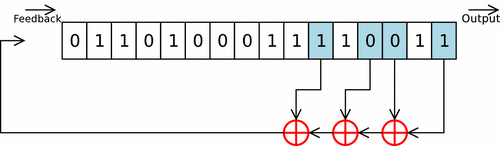
\includegraphics{images/Lfsr}
		\caption{Exemple d'un registre à décalage à rétroaction linéaire (LFSR)}
		\label{fig:lfsr}
	\end{figure}
	Le bit calculé est réinjecté dans le registre.
	\subsubsection{Chiffrement par flux A5/1}
	Le chiffrement A5/1 a été utilisé dans la communication GSM depuis 1994. Il a
	été cassé en 2009.
	\par
	La communication utlise deux flux (montant et descendant). Chaque flux
	transmet 114 \textit{bits} chiffrés dans un bloc de 4,6 \textit{ms}. Un
	générateur aléatoire produit 228 \textit{bits}. Ensuite l'algorithme utilise
	trois LFSR et une clé de session K entre le portable et l'antenne. Chacun des
	trois LFSR utilise un \textit{clocking bit} lui indiquant s'il peut se décaler
	 ou pas. Cet horodotage irrégulier permet d'introduire une confusion. Un LFSR
	est autorisé à se décaler si la valeur de son bit d'horloge est majoritaire
	parmi celles des trois LFSR.
	\begin{figure}[!ht]
		\centering
		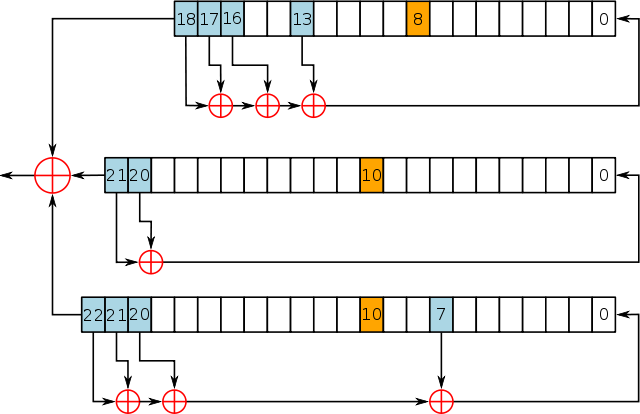
\includegraphics[width=1\textwidth]{images/Lfsra51}
		\caption{Utilisation de LFSR par l'algorithme de chiffrement A5/1 (bit
		d'horloge est en orange)}
		\label{fig:lfsra51}
	\end{figure}
	\subsection{Chiffrement par bloc}
	Le principe est de découper le texte claire en \textbf{blocs de taille
	identique} et d'effectuer un chiffrement itératif sur chaque bloc. La
	longueur des clés doit être supérieure à 128 \textit{bits}. Cet algorithme
	utilise une fonction interne \textit{F} appliquée à chaque tour de chiffrement
	 qui utilise une combinaison de « boîtes » et de OUEX pour effectuer une
	permutation linéaire (\textit{P-Box}) et une substitution non-linéaire
	(\textit{S-Box}).
	\par
	\textit{P-Box} utilise une matrice pour permuter les bits. Par contre
	\textit{S-Box} effectue une substitution de bits d'entrée en fonction d'un
	tableau. Cette substituion peut également servir pour compresser des données
	car la sortie de la substitution peut être d'une longueur inférieure à
	l'entrée (\textit{S-Box 6/4} du chiffrement DES).
	\subsubsection{Réseau de Feistel}
	Lors du chiffrement on découpe le bloc en deux parties $(L_{0}, R_{0})$ et à
	chaque tour $i = 0...n$ on effectue :
	\[ L_{i+1} = R_{i} \]
	\[ R_{i+1} = L_{i} \oplus F(R_{i}, K_{i}) \]
	Le message chiffré obtenu est $(R_{n+1}, L_{n+1})$.
	\begin{figure}[!ht]
		\centering
		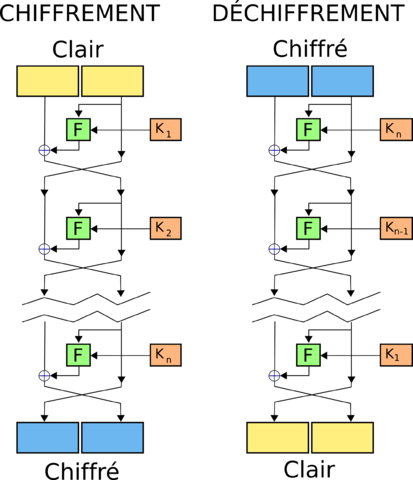
\includegraphics[scale=0.9]{images/feistel}
		\caption{Déroulement de chiffrement respectivement de déchiffrement de
		Feistel}
		\label{fig:feistel}
	\end{figure}
	\subsubsection{Chiffrement DES}
	C'est un chiffrement symétrique par blocs de 64 \textit{bits}. Les clés sont
	de 58 \textit{bits}. Les 6 \textit{bits} restant sont pour le contrôle de
	parité. L'algorithme effectue 16 itérations de chiffrement.
	\begin{figure}[!ht]
		\centering
		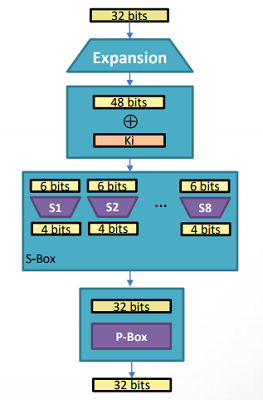
\includegraphics{images/des}
		\caption{Fonction F utilisé par le chiffrement DES}
		\label{fig:des}
	\end{figure}
	\subsubsection{Chiffrement AES}
	L'algorithme AES utilise des blocs et des clés de 128 à 256 \textit{bits} et
	effectue respectivement 10, 12 et 14 itérations. \textit{A contrario} de DES
	il n'est pas basé sur un réseau de Feistel. AES est encore considéré sûr de
	nos jours. La seule attaque possible est par force brute.
	\par
	4 blocs de fonctions sont utilisés (\textit{SubBytes, ShiftRows, MixColumns,
	AddRoundKey}) ainsi que 10 itérations. La clé de chaque itération est dérivée
	par fonction successive (\textit{X, S-Box, OUEX}).
	\par
	\textit{SubBytes} substitue 16 \textit{octets} correspondant à 128
	\textit{bits} selon une table prédéfinie.
	\par
	\textit{ShiftRows} effectue un décalage variable des octets selon la ligne.
	\par
	\textit{MixColumns} multiple chaque colonne par une matrice prédéfinie.
	\par
	\textit{AddRoundKey} calcule un OUEX avec la clé.
	\subsubsection{Contraintes des algorithmes de chiffrement par bloc}
	\begin{itemize}
		\item taille de blocs limitée
		\item taille de clés limitée
		\item impossible pour de grandes quantités de données
	\end{itemize}
	Plusieurs solutions existent :
	\begin{itemize}
		\item chaînage de blocs
		\item utiliser un vecteur d'initialisation
		\item dictionnaire de codes (\textit{Electronic CodeBook}, ECB, $Mc_{i} =
		F(Md_{i}, K)$) : séparation de données par morceau qui sont chiffrés
		séparément avec la même clé, possibilité de comparer les textes chiffrés et
		faire une analyse statistique
		\item enchaînement de blocs (\textit{Cipher Block Chaining}, CBC, $Mc_{1} =
		F(Md_{1} \oplus IV, K), Mc_{i} = F(Mc_{i-1} \oplus Md_{i}, K)$) : effectue
		un OUEX avec le bloc qui précède avant le chiffremenr par bloc, utilise un
		vecteur d'initialisation \textit{IV} aléatoire et unique
		\item chiffrement à rétroaction (\textit{Cipher Feedback}, CFB, $Mc_{1} =
		F(IV, K) \oplus Md_{1}, Mc_{i} = F(Mc_{i-1}, K) \oplus Md_{i}$) : vecteur
		d'initialisation est chiffré avec la clé, le texte clair n'est pas
		directement chiffré par un bloc, en disposant de la clé il est possible de
		déchiffrer jusqu'à l'avant dernier bloc
		\item chiffrement à rétroaction de sortie (\textit{Output Feedback}, OFB,
		$Mc_{1} = F(IV, K) \oplus Md_{1}, Mc_{i} = F(IV, K)_{i-1} \oplus Md_{i}$) :
		vecteur d'initialisation est chiffré avec la clé, la clé précédente est
		utlisée pour chiffrer la clé suivante
	\end{itemize}
	\subsection{Partage de secret}
	Le problème du chiffrement symétrique à grande échelle est l'échange de la
	clé qui doit être absolument sûre. De plus entre chaque paire de correspondant
	 il faut une clé.
\end{document}
